\documentclass[12pt]{article}

\usepackage{times}
\usepackage{graphicx}
\usepackage{datetime}
\usepackage[utf8]{inputenc}
\usepackage[slovene]{babel}
\usepackage[font=]{caption}

\newdateformat{MMYYYYdate}{\monthname[\THEMONTH] \THEYEAR}
\title{RIPtide - Univerzalno orodje za konfiguracijo omrežij}
\author{Jurij Fortuna, G 3. a}
\date{\MMYYYYdate\today}

\begin{document}

\begin{center}
	\thispagestyle{empty}
	
\includegraphics[scale=1]{slike/vegova.png}

	\vspace{\fill}
	Seminarska naloga pri predmetu računalništvo

	\Huge{RIPtide - Univerzalno orodje za konfiguracijo omrežij}

	\normalsize
	\vspace{\fill}

	Mentor: Marko Kastelic, prof. \hfill Avtor: Jurij Fortuna , G 3. a\\
	\null
	Ljubljana, \MMYYYYdate\today
\end{center}
\newpage

% Povzetek
\section*{Povzetek}
Seminarska naloga opisuje matematični vidik delovanja cyclic redundancy
check-a, ob tem pa na kratko opiše tudi matematične pojme, kot so konča
polja in polinomi. Pokaže tudi, kako CRC implementirati z
logičnim vezjem.\\\\
\textbf{Ključe besede:} CRC, končna polja, polinomi, logična vezja, digitalna
komunikacija\\

\section*{Abstract}
\foreignlanguage{english}{
	This paper describes mathematical part of cyclic
	redundancy check, while at the same time depicts mathematical terms like finite
	fields and polynomials. The paper shows how to implement CRC with logic circuit.\\
	\\
	\textbf{Keywords:} CRC, finite fields, polynomials, logic circuits, digital
	communication
}
\newpage

% Kazalo
\tableofcontents
\newpage

% 1. Uvod
\section{Uvod}
Ideja za razvoj RIPtide-a se je pojavila, ko sem bil med konfiguracijo
domačega omrežja prisiljen uporabljati tri različne programske opreme,
različnih proizvajalcev. Med sabo so se nemalo razlikovale in so bile
po večini nestabilne. Zato sem se odločil razviti generično programsko
opremo za konfiguracijo omrežij. Deluje na principu
“vtičnikov” (t.i. Shedov) za posamezne kose omrežne opreme.\\\\\\

\begin{center}
	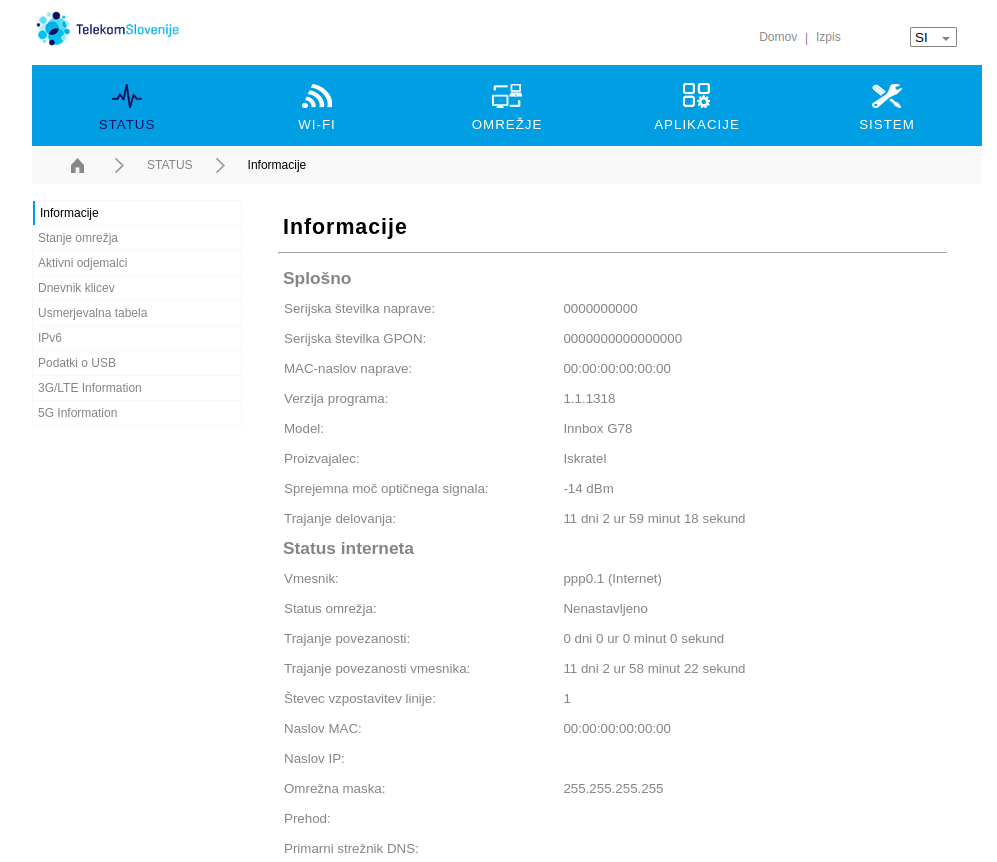
\includegraphics[scale=0.5]{slike/telekom.png}
	\captionof{figure}{Primer konfiguracijske strani za usmerjevalnike Telekoma Slovenije}
\end{center}
\newpage

% 2. Tehnologije
\section{Uporabljene tehnologije}
Tako Shedi, kot tudi RIPtide so napisani v Javi. Java omogoča dinamično
nalaganje modulov ob zagonu navideznega stroja, tudi iz zapakiranih jar
datotek. Sam RIPtide je zgrajen iz dveh glavnih delov: osprednega dela 
in aplikacijskega programskega vmesnika (v nadaljevanju API).
Poleg tega velja omeniti Shede, ki jih lahko razvije kdorkoli z uporabo
RIPtide API-ja.

\subsection{Ospredni del}
Ospredni del je odgovoren za konfiguracijo RIPtide-a, nalaganje Shedov
in rokovanje z uporabnikovimi napravami ter pripadajočimi poverilnicami.

\subsubsection{Konfiguracija}
Uporabnik lahko svoje naprave shrani, in si s tem prihrani čas za morebitno
kasnejšo konfiguracijo. Poleg tega RIPtide omogoča spremembo barve vmesnika
po svoji želji.

\subsubsection{Nalaganje Shedov}

\subsubsection{Upravljanje poverilnic}
Za konfiguracijo večine omrežnih naprav je potrebna avtorizacija.
RIPtide uporabnikom omogoča varno shranjevanje poverilnic na njihovem
sistemskem keyringu (sistem za varno hranjenje gesel). Poverilnice so ob
povezavi na napravo prek API-ja podani Shedu, kar pomeni, da se razvijalci
teh ne rabijo ukvarjati z varnim hranjenjem poverilnic.
\newpage

\end{document}